\documentclass[a4paper,12pt]{llncs}
\usepackage[top=75pt, bottom=75pt, left=85pt, right=85pt]{geometry}

\usepackage{subfigure}
\usepackage{amssymb}
\usepackage{amsmath}
\setcounter{tocdepth}{3}
\usepackage{graphicx}
\usepackage{soul,color}
\usepackage{url}
\usepackage{algorithm}
%\usepackage{enumitem}
\newcommand{\keywords}[1]{\par\addvspace\baselineskip
\noindent\keywordname\enspace\ignorespaces#1}
\newcommand{\ie}{i.e.} 
\newcommand{\eg}{e.g.} 
\newcommand{\et}{et al. }

\begin{document}
\title{Weekly Report -- 51}
\author{Xiufeng Liu}
\institute{University of Waterloo, CA\\
\email{xiufeng.liu@uwaterloo.ca}
}
\maketitle
\section{Introduction}

\section{Water Demand Forscasting Issues}

\subsection{Forcasting Models}

\subsection{Time Scales}

\subsection{Water Demand Patterns}

\section{Exploratory Analysis of Water Consumption Data}
\subsection{Water Use Distributed over  Customer Types}
The water consumption data is from  Abbotsford  city, British Columnbia, Canada from September 1, 2012 to August 31, 2013. Daily and hourly time-series data were collected from 25,294 customers,  distributed in six customer groups (see Figure~\ref{fig:customergroups}). There are 2013 215,172,496 data points in total for the hourly time-seriels data, and 9,232,310 data points for the daily time-series data (roughly 10GB in total). The residential customers are discriminated according to the house types, which are single family residential (SFRES) and multifamily residential (MFRES). As shown, the single family residential has the biggest share (79.61\%).

The climate data at the same period were downloaded from from Environment Canada (https://weather.gc.ca). The data contains the weather temperature at hourly resolution, and the rainfall at daily resolution.
\begin{figure*}[htp]
\centering
\begin{minipage}[b]{0.45\linewidth}
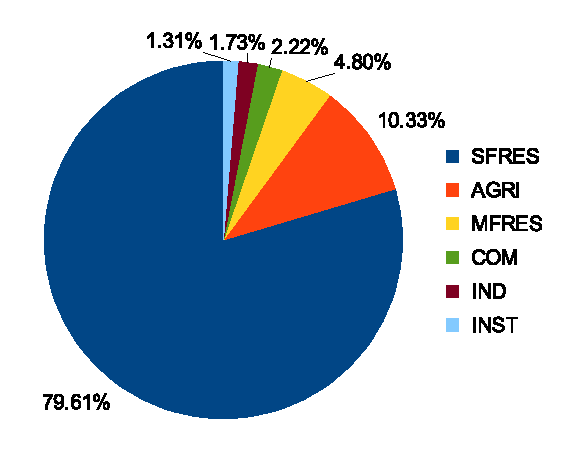
\includegraphics[width=0.9\textwidth]{images/watercustomergroups}
\vspace{-5pt}
\caption{Sizes of customer group}
\label{fig:watercustomergroups}
\end{minipage}
\begin{minipage}[b]{0.5\linewidth}
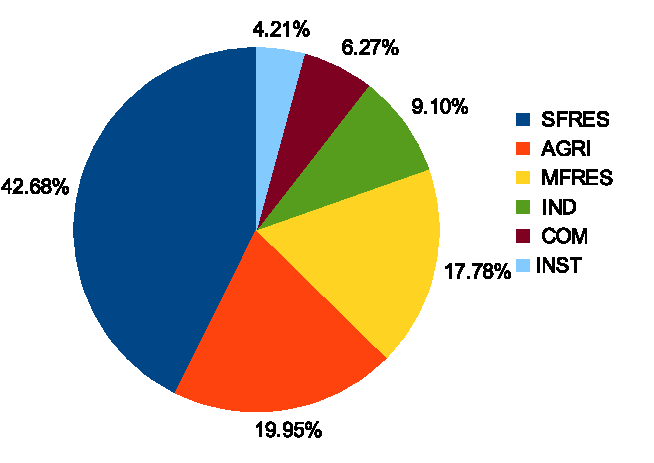
\includegraphics[width=0.9\textwidth]{images/waterconsumptiondist}
\vspace{-5pt}
\caption{Water consumption distribution}
\label{fig:waterconsumptiondist}
\end{minipage}
\end{figure*}
\begin{table}[h]
\centering
\caption{Sizes of customer types and the water consumption}
\begin{tabular}{p{2cm}p{2cm}p{2cm}p{2cm}p{2cm}p{2cm}}
\hline
                        & \multicolumn{2}{c}{Customer Types}                            &                      & \multicolumn{2}{c}{Water Consumption}                                    \\ \cline{2-3} \cline{5-6} 
                        & \multicolumn{1}{c}{Size} & \multicolumn{1}{c}{Percentage, \%} & \multicolumn{1}{c}{} & \multicolumn{1}{c}{Consumption, $m^3$} & \multicolumn{1}{c}{Percentage, \%} \\ \hline
\textbf{SFRES}          & 20,136                   & 79.61                              &                      & 5,158,189.4                         & 42.68                              \\
\textbf{AGRI}           & 2,612                    & 10.33                              &                      & 2,411,693.3                         & 19.95                              \\
\textbf{MFRES}          & 1,215                    & 4.80                               &                      & 2,148,880.4                         & 17.78                              \\
\textbf{COM}            & 561                      & 2.22                               &                      & 758,081.3                           & 6.27                               \\
\textbf{IND}            & 438                      & 1.73                               &                      & 1,099,533.5                         & 9.10                               \\
\textbf{INST}           & 332                      & 1.31                               &                      & 509,298.9                           & 4.21                               \\ \hline
\textit{\textbf{Total}} & 25,294                   & 100                                &                      & 12,085,676.9                        & 100                                \\ \hline
\end{tabular}
\label{tab:custgroupandconsump}
\end{table}


\begin{figure}[htp]
\centering
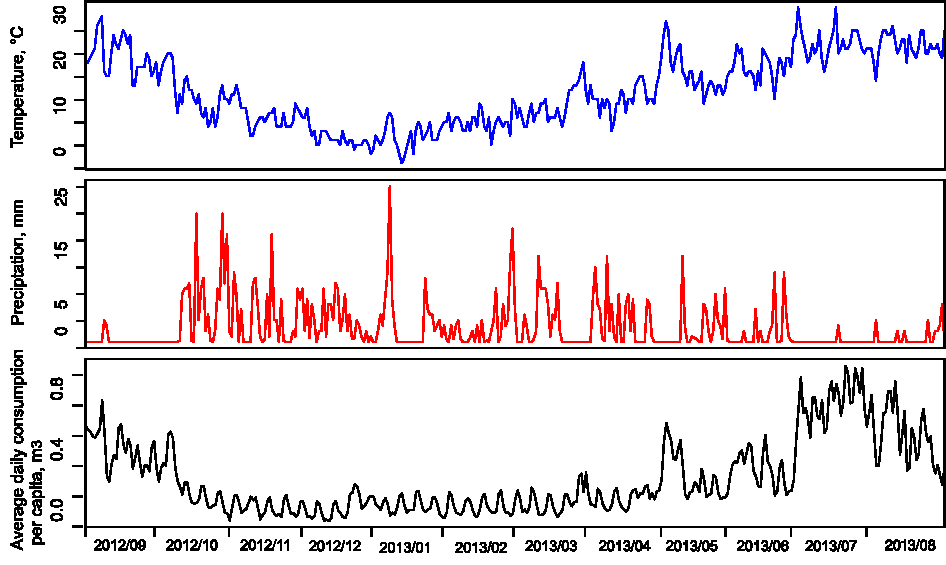
\includegraphics[width=0.9\textwidth]{images/weathervariableinwaterdemand}
\caption{The average daily profile of residential water consumption}
\label{fig:dailyprofile}
\end{figure}

\subsection{Residential Water Use in Abbotsford}
Approximately two-thirds of the water used in Phoenix is for residential purposes, 51\% by the residents of single-family homes. In a spatially weighted regression analysis of single-family residential water demand at the census tract level, Wentz and Gober (2007) found that four variables--average household size, the percent of homes with a swimming pool, average lot size, and average percent of lots covered with mesic (turf) vegetation—explained more than 80\% of the spatial variation in metered water use. Larger household size increases indoor water use for such purposes as toilet flushing, showers, laundry, and dishwashing, although Arbu\'{e}s et al. (2003) note the tendency for less-than-proportional increases in use because of economies of
scale in water use. Swimming pools, lot size, and vegetation type account for outdoor use from pool evaporation and garden irrigation. We anticipate that residential water use is climate sensitive because of the
heavy reliance on outdoor uses in Phoenix’s water portfolio.

In a study of the effect of the urban heat island on
water use in Phoenix, Guhathakurta et al. (2005) ex-
amined the spatial effects of June nighttime tempera-
ture on residential water use, controlling for the pres-
ence of pools, vegetation type, size of house and lot,
number of residents, and other socioeconomic, demo-
graphic, and housing variables. The effect of tempera-
ture was statistically significant, and the regression co-
efficient indicated that an increase of 1°C resulted in an
increase in household water use of 4.61 kL annually. In
an environment in which the typical residence uses
more than 600 kL of water, this constitutes 0.77% of
annual use for every 1°C of urban heating. With the
heat-island effect exceeding 6°C, residential water use
can be affected by over 4.5%.


We show the daily time-series of the residential water usage in Figure~\ref{sfrestimeseries}. we could observer that the water usage shows periodicity in the days of a week. From Monday--Friday, the consumptions are lower than the weekend, and the holidays, propably for the reason that in the weekend and holiday people stays more time at home, thus use more water. In addition, we could observer that in summer time (May - October) the consumption are higher than winter time (November--April) which is probably due to the temperature effect. For example,  households grow the flowers in outdoors in summer, which need to water the flowers,  wash the care, or fill the swimming pools. Another climate effect we might consider is the effect of rainfall. For example, due to the rainfall, the water consumption might be reduced, \eg, people can save the water for watering the flowers in outdoor.


\begin{figure}[htp]
\centering
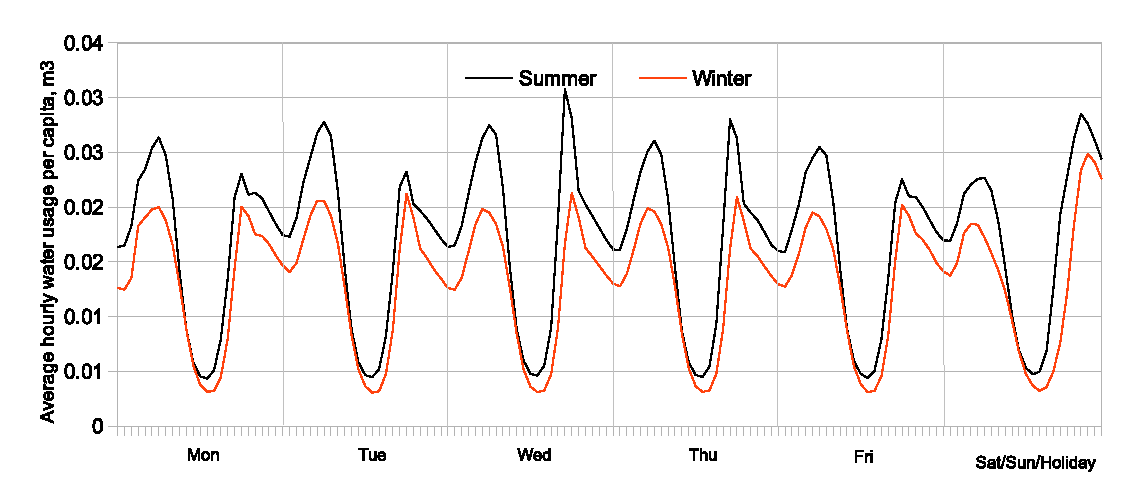
\includegraphics[width=1\textwidth]{images/avgweeklyprofile}
\caption{The average weekly profile of single family residential water consumption}
\label{fig:dailyprofile}
\end{figure}



\section{Model for Residential Water Demand Forecasting}
\subsection{Basis for Water Demand Forecasting}
Planning for decision making forms the basis for forecasting in the
water sector. To this end, a set of water demand forecasting liter-
ature differentiates forecast practice by the level of planning asso-
ciated with the forecast (Gardiner and Herrington 1990), or in
accordance with the forecast horizon (Billings and Jones 2008).
In terms of planning level, all water demand forecasting exercises
can be used for strategic, tactical, or operational decision making.
These concern decisions for capacity expansion, investment plan-
ning and system operation, management, and optimization, respec-
tively. In terms of forecast horizon, water demand forecasting can
be categorized as either long-term, medium-term, or short-term,
with these horizons being reflective of the planning levels, respec-
tively (Alvisi et al. 2007; Ghiassi et al. 2008; Jain et al. 2001).
No generally accepted time frame exists for these horizons.
Billings and Jones (2008) contain different time horizons on what
constitutes long-term, medium-term, and short-term forecasts. One
such definition classifies forecasts spanning more than two years as
long-term, those from three months to less than two years as medium-
term, and forecasts for one to three months as short-term. This con-
trasts with Gardiner and Herrington (1990), in which these categories
are classified as annual forecasts for 10 years or more (long-term),
annual forecasts for 1 to less than 10 years (medium-term), and hourly
to monthly forecasts up to a year (short-term). In terms of reported
research, Ghiassi et al. (2008) prepared monthly demand forecasts
for two years, weekly demand forecasts for six months and daily
demand forecasts for two weeks, and characterize these as long-term,
medium-term, and short-term, respectively. In Table 1, we follow
Gardiner and Herrington (1990) in categorizing the forecast horizon
by planning level and summarize how these relate to the decision
problem and the forecast periodicity

In the drinking water industry, many variables are considered
influential in determining water demand. These range from socio-
economic to various derivatives of weather-related variables. Ex-
amples of these weather-related variables and how they are used
can be found in Coomes et al. (2010) and Brekke et al. (2002).
Although “A good understanding of the factors influencing demand
and reliable estimates of the parameters describing demand behav-
ior and consumption patterns are prerequisites [to a good forecast]”
(Burney et al. 2001), the enormity of these variables can create frus-
tration for water utility mangers. As an illustration of the size and
variability of the variables that can be considered, we refer to a
report prepared for the Water Research Foundation by Coomes et al.
(2010), in which the authors tested the effect of 26 variables on
average daily water use for 293 residential customers of the Louis-
ville Water Company. The availability and choice of these indepen-
dent variables can also influence the forecasting models used. For
instance, whereas population projections and per capita demand are
the drivers for unit rate models, these have no consideration when
exponential smoothing or Box-Jenkins models are formulated

We model the water consumption, $W_i$, into base load and seasonal load, which is as follows:
\begin{equation}
D_i = B_i + S_i 
\end{equation}

\subsection{Base load}
The base load represents the weather insensitive portion of the total water use. The base load mainly are due to the use of daily use of living, such as drinking, toilet, bath and washing. The base use are unlikely to change abruptively, but might change slowly, \eg, placing more water efficient appliance such as new washing machine.  Therefore, the base use is assumed to be a fixed percentiled consumption of hourly flows in household for weekdays and weekends/holidays. We use 10 percentiled water usage as the base load, also adopted by \cite{zhou2002}.



\subsection{Daily Seasonal Load}
The seasonal load represents the weather sensitive portion of the total use, \ie, $S_i=D_i - B_i$. We use the use the periodic Auto-Regression with eXogenous variables (PARX) \cite{omid} (weather temperature and waterfall) to model the seasonal load. We use  the week as the period, and the weekdays as the seasons. The water consumption can be modeled as:
\begin{equation}
S_t = \sum_{i=0}^{p} \phi_{s,i} S_{i-p} + \beta_s H(T_t) + \psi_s G(R_t) + \epsilon_s,  \quad t \in s
\end{equation}
where $Y_t$ represents the water consumption at a particular day $t$ in a week; $t$ is the weekday whose values are $0,...,6$ representing Sunday, Monday, ..., Saturday; $p$ is the order of auto-regression; $s$ is the season index; $\phi_{s,i}, \beta_s, \psi_s$ are the coeffcients, and $\epsilon_s$ is the white noise;  $H(T_t)$ and $G(R_t)$ are the functions of weather temperature and rainfall effects, and defined as:

\[ H(T_t) = \left\{ 
  \begin{array}{l l}
    T_t - \tau & \quad T_t>\tau\\
    0 & \quad \text{Otherwise}
  \end{array} \right.\]

\[ G(R_t) = \left\{ 
  \begin{array}{l l}
    \gamma  & \quad R_t>\gamma\\
    R_t & \quad  \text{Otherwise}
  \end{array} \right.\]

where $T_t$ is the temperature at the week day $t$, and $\tau$ the thredhold of temperature effect; $R_t$ is the preciptation at the week day $t$, and $\gamma$ is the thredhold. 


\subsection{Hourly Seasonal Load}
-- No hourly rainfall data


\section{Results}
\subsection{Accuracy of the forcasting model}
{\bf Evaluation.} We now use daily single family residential (SFRES), and weather data to compute the coefficients. We set the temperature thredhold value $\tau$ as 20 celsius degree, and the thredhold value of rainfall $\gamma$ as 1 mm preciptation.



\medskip
\begin{thebibliography}{1}

\bibitem{zhou2002}
Zhou, S. L., T. A. McMahon, A. Walton, and J. Lewis. "Forecasting operational demand for an urban water supply zone." Journal of Hydrology 259, no. 1 (2002): 189-202.

\bibitem{ibmbenchmark}
Ten Million Meters Scalable to One Hundred Million Meters for Five Billion Daily Meter Readings. Sept. 2011.

\bibitem{omid}
Ardakanian, O., Koochakzadeh, N., Singh, R. P., Golab, L., and Keshav, S. (2014). Computing Electricity Consumption Profiles from Household Smart Meter Data. In EDBT/ICDT Workshops (pp. 140-147).

\end{thebibliography}



\end{document}
